\documentclass{article}
\usepackage{graphicx}
\usepackage{amsmath}
\usepackage{float}
\usepackage{subfigure}
\usepackage{enumerate}
\usepackage{geometry}
\usepackage{float}
\usepackage{cite}
\usepackage{color}
\usepackage{listings}

% \usepackage{geometry}
% \geometry{a4paper,scale=0.8}

\usepackage{appendix}

\title{21cm intensity mapping with FAST}
\author{Zerui Liu}
\date{\today}

\begin{document}
\maketitle
\tableofcontents
\section{Evolution of 21cm cosmic hydrogen signal}
The Big Bang model has now helped us to have a more mature understanding of the evolutionary history of the universe. Current observations have covered the evolution of the universe from about 400,000 years after the Big Bang to the present day. However, we still lack observational evidence for the first billion years of the universe's evolution, when the first stars and planets formed, to figure out what happened during this time. Meanwhile, as the afterglow of the Big Bang, the CMB gives us a message of the early evolution of the universe. CMB and the gas decoupled 400,000 years after the Big Bang when the universe cooled sufficiently for photons and electrons to combine to form neutral hydrogen at that time. Radiation from this time is able to reach us directly and provide a snapshot of early universe.

Connecting these two periods of universe represents a huge challenge. Currently perturbation theory is widely used to explain the connection of these two periods. The observation of CMB reveals that the early universe was inhomogeneous at the level of 1 part in 100,000. As evolution progresses, gravity causes these perturbations to grow into larger nonlinear structures and further collapse into other structures such as sheets, filaments and halos. On the basis of these nonlinear structures, galaxies form by the collapse and cooling of the gas and reach the densities needed for star formation.

In order to probe the evolutionary details of this period, the method of 21 cm intensity mapping can be used to replace the traditional observation of galaxies. This 21 cm line is produced by the hyperfine splitting caused by the interaction between electron and proton magnetic moments. Plotting the intensity distribution of the 21-cm line provides insight into the distribution of neutral hydrogen in the early universe. Hydrogen is ubiquitous in the universe, accounting for 75\% of the mass of gas present in the intergalactic medium (IGM). As such, it provides a convenient tracer of the properties of this gas and of the major milestones in the first billion years of the history of the Universe.

Figure \ref{historyofHI} shows the evolution of 21cm signal with cosmic time. The bottom panel shows the average strength of 21cm global signal while the top panel shows the fluctuation of 21cm signal arising
from variation in density. In the "dark age" of the universe, the first structures begin to grow from the seed inhomogeneties probably caused by quantium 
fluctuations. The 21cm absorption signal caused by the cold gas can be seen at this period. The $Ly\alpha$ photons produced by the first forming stellars and galaxies lead to a strong coupling between the gas temperature and the 21 cm line excitation. Initially, this coupling leads to a strong global absorption signal. This absorption signal is spatially inhomogeneous due to the strong clustering properties of the first generation galaxies. Afterwards, the X-rays from the galaxy heat up the gas, resulting in an emission signal of 21 cm lines. Finally, the X-rays produced by the galaxy gradually cause the gas to ionize gradually, leading to the creation of voids in the spatial distribution of the 21cm emission signal. Eventually, the gas is all ionized and the 21cm global signal disappears.

\begin{figure}
    \centering
    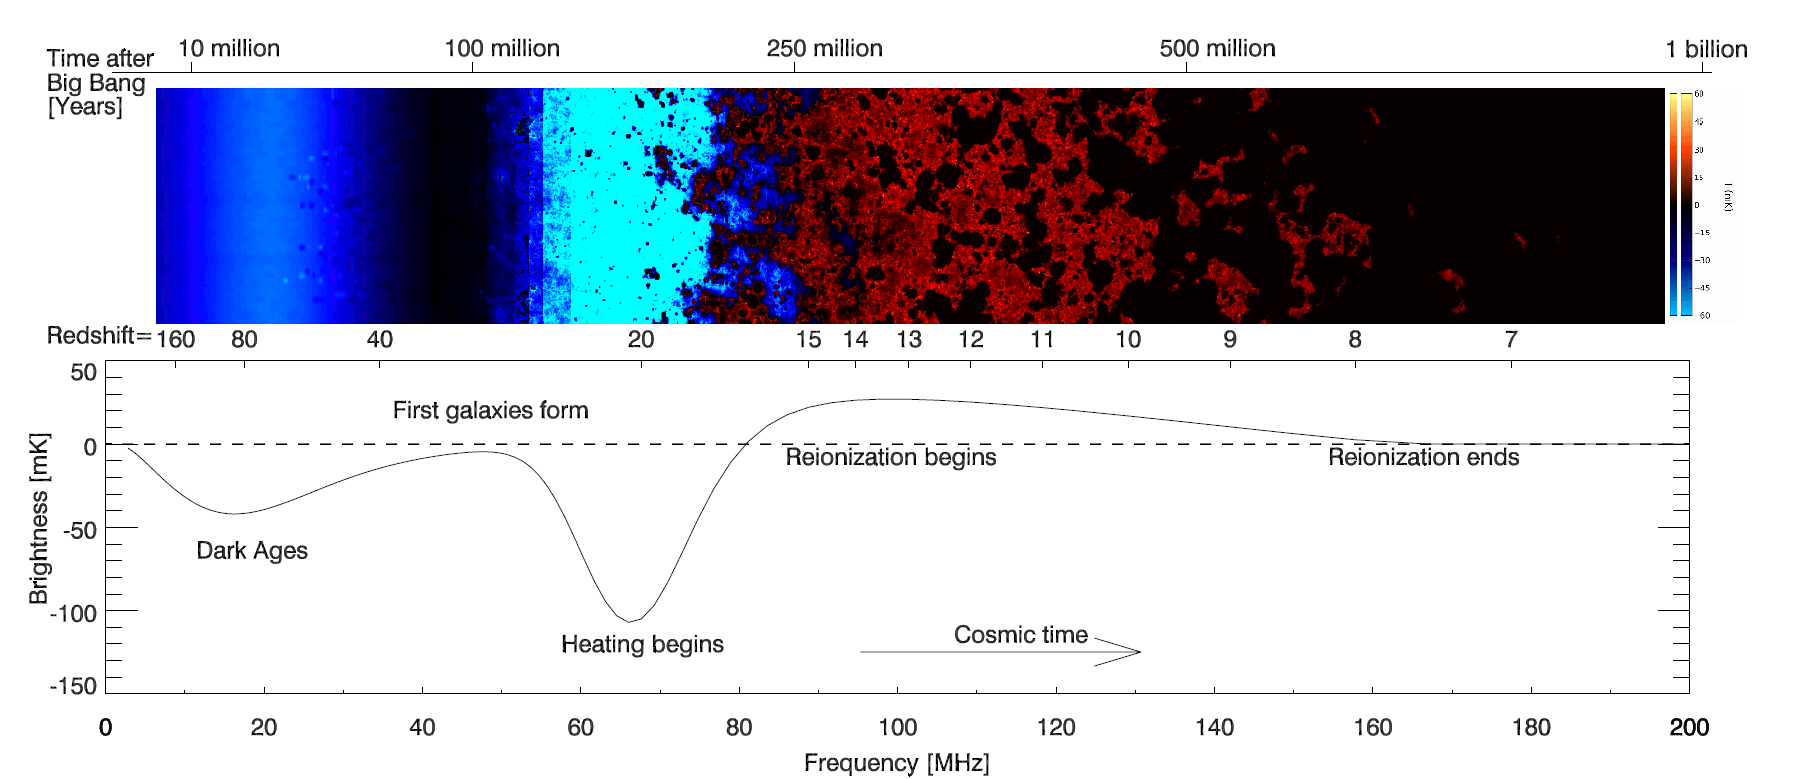
\includegraphics[scale=0.3]{history1.png}
    \caption{}
    \label{historyofHI}
\end{figure}

The stages of each evolutionary process can be discussed in detail according to the redshift interval in which each stage occurs, roughly as follows:
\begin{itemize}
    \item $200<Z<1000$: The residual electron component after the proton-electron recombination can couple the gas and the CMB together. The high-intensity collisional coupling makes the spin temperature $T_{S}$ and the CMB temperature $T_{\gamma}$ equal, when the bright temperature of the 21cm line is 0 and there is no detectable 21cm signal.
    \item $40<z<200$: The gas cools adiabatically as the universe expands and the kinetic temperature follows $T_K\propto (1+z)^2$, leading to a kinetic temperature below the CMB temperature $T_{\gamma}$. The bright temperature $T_b < 0$ and exhibits an absorption signal. 
    \item $z_*<z<40$: As the expansion of the universe continues, the density of the gas decreases, the strengtrh of the collisional coupling decreases, and the radiative coupling brought about by the CMB makes $T_S=T_{\gamma}$, which is no detectable 21cm signal.
    \item $z_\alpha < z < z_*$: At redshift $z_*$, stars and galaxies begin to form as the first sources of radiation and start emitting $Ly_\alpha$ photons and X-rays. 
\end{itemize}

\section{Physical mechanisms of intensity of the 21 cm line}

\section{Intensity mapping with FAST}

\end{document}